\documentclass[tikz,border=8pt]{standalone}
\usepackage{amsmath}
\usetikzlibrary{arrows.meta,positioning,fit,calc}

\begin{document}
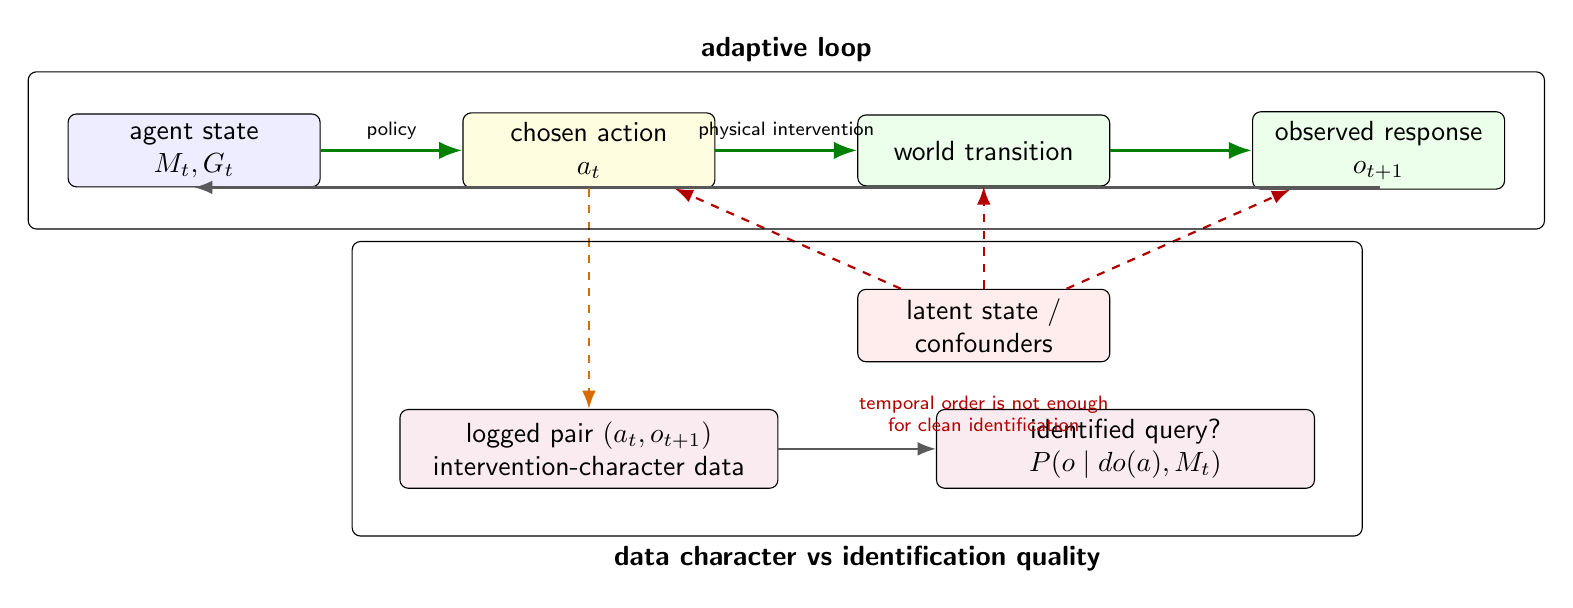
\begin{tikzpicture}[
  font=\sffamily,
  box/.style={draw, rounded corners=3pt, align=center, minimum width=32mm, minimum height=9mm, fill=white},
  wide/.style={draw, rounded corners=3pt, align=center, minimum width=48mm, minimum height=10mm, fill=white},
  arrow/.style={-Latex, thick, draw=black!65},
  good/.style={-Latex, very thick, draw=green!50!black},
  warn/.style={-Latex, thick, dashed, draw=orange!85!black},
  bad/.style={-Latex, thick, dashed, draw=red!70!black},
  note/.style={align=center, font=\sffamily\scriptsize}
]

\node[box, fill=blue!7] (agent) {agent state\\$M_t,G_t$};
\node[box, right=18mm of agent, fill=yellow!12] (action) {chosen action\\$a_t$};
\node[box, right=18mm of action, fill=green!8] (world) {world transition};
\node[box, right=18mm of world, fill=green!8] (obs) {observed response\\$o_{t+1}$};
\node[box, below=13mm of world, fill=red!7] (hidden) {latent state /\\confounders};
\node[wide, below=28mm of action, fill=purple!8] (log) {logged pair $(a_t,o_{t+1})$\\intervention-character data};
\node[wide, right=20mm of log, fill=purple!8] (id) {identified query?\\$P(o\mid do(a),M_t)$};

\draw[good] (agent) -- node[above, note] {policy} (action);
\draw[good] (action) -- node[above, note] {physical intervention} (world);
\draw[good] (world) -- (obs);
\draw[arrow] (obs.south) |- (agent.south);

\draw[warn] (action) -- (log);
\draw[arrow] (log) -- (id);

\draw[bad] (hidden) -- (action);
\draw[bad] (hidden) -- (world);
\draw[bad] (hidden) -- (obs);
\node[note, below=3mm of hidden, text=red!70!black]
  {temporal order is not enough\\for clean identification};

\node[draw, rounded corners=3pt, fit=(agent)(action)(world)(obs), inner sep=5mm,
  label={[font=\sffamily\bfseries]above:adaptive loop}] {};
\node[draw, rounded corners=3pt, fit=(log)(id)(hidden), inner sep=6mm,
  label={[font=\sffamily\bfseries]below:data character vs identification quality}] {};

\end{tikzpicture}
\end{document}
